\subsection{Taxi Manager}
\begin{figure}[H]
	\centering
	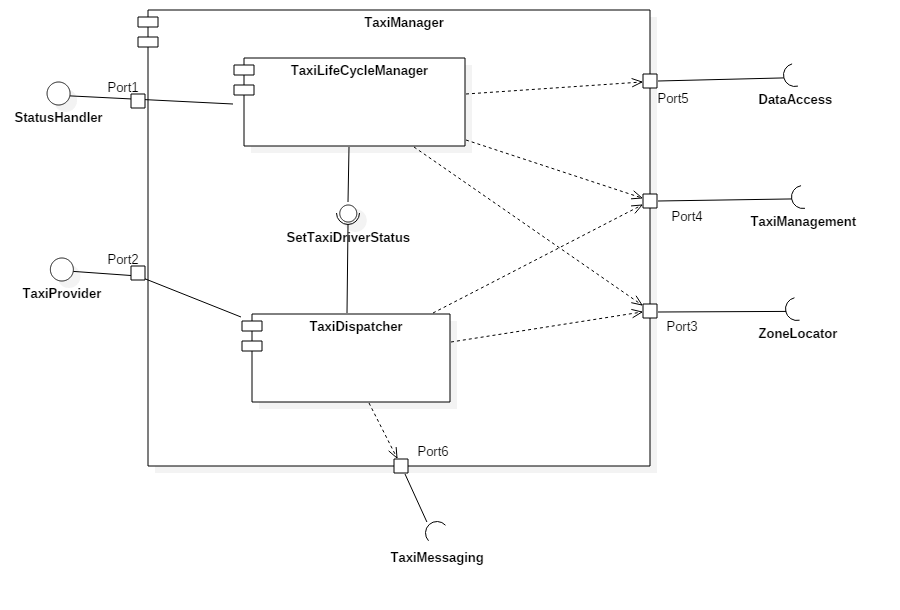
\includegraphics[scale=0.5]{../"Analysis Documents"/components/taxiManager}
	\label{fig:taximanager}
	\caption{Taxi Manager internal structure}
\end{figure}
\subsubsection{Provided interfaces}
\begin{table}[H]
	\begin{longtable}{| p{0.3\textwidth} | p{0.3\textwidth} | p{0.4\textwidth} |}
		\hline
		\textbf{Provided Interface} & \textbf{Dedicated user} & \textbf{Description} \\ \hline
		StatusHandler & The Taxi driver's mobile application & Allows the taxi driver to set himself as 'Available' and 'Not Available'. Plus, it is used from the application to communicate the current location \\ \hline
		TaxiProvider & Ride Manager component & Given a location, it provides a taxi (if the correspondent queue is not empty and one taxi accepts) \\ \hline
	\end{longtable}
	\caption{Taxi manager: provided interfaces}
	\label{tab:taximanager:providedInterfaces}
\end{table}
\subsubsection{Required interfaces}
\begin{table}[H]
	\begin{longtable}{| l | p{.80\textwidth} |}
		\hline
		\textbf{Required Interface} & \textbf{Description and usage} \\ \hline
		ZoneLocator & Retrieves the correspondent zone of a location \\ \hline
		DataAccess & Save the information of the taxi driver status \\ \hline
		TaxiManagement & It communicates to the data structure containing the taxi drivers, whether to add, remove or retrieve them. \\ \hline
	\end{longtable}
	\caption{Taxi manager: required interfaces}
	\label{tab:taximanager:requiredInterfaces}
\end{table}
